\documentclass{beamer}

\pdfmapfile{+sansmathaccent.map}


\mode<presentation>
{
	\usetheme{Warsaw} % or try Darmstadt, Madrid, Warsaw, Rochester, CambridgeUS, ...
	\usecolortheme{seahorse} % or try seahorse, beaver, crane, wolverine, ...
	\usefonttheme{serif}  % or try serif, structurebold, ...
	\setbeamertemplate{navigation symbols}{}
	\setbeamertemplate{caption}[numbered]
} 


%%%%%%%%%%%%%%%%%%%%%%%%%%%%
% itemize settings


%%%%%%%%%%%%%%%%%%%%%%%%%%%%
% itemize settings

\definecolor{myhotpink}{RGB}{255, 80, 200}
\definecolor{mywarmpink}{RGB}{255, 60, 160}
\definecolor{mylightpink}{RGB}{255, 80, 200}
\definecolor{mypink}{RGB}{255, 30, 80}
\definecolor{mydarkpink}{RGB}{155, 25, 60}

\definecolor{mypaleblue}{RGB}{240, 240, 255}
\definecolor{mylightblue}{RGB}{120, 150, 255}
\definecolor{myblue}{RGB}{90, 90, 255}
\definecolor{mygblue}{RGB}{70, 110, 240}
\definecolor{mydarkblue}{RGB}{0, 0, 180}
\definecolor{myblackblue}{RGB}{40, 40, 120}

\definecolor{myblackturquoise}{RGB}{5, 53, 60}
\definecolor{mydarkdarkturquoise}{RGB}{8, 93, 110}
\definecolor{mydarkturquoise}{RGB}{28, 143, 150}
\definecolor{mypaleturquoise}{RGB}{230, 255, 255}
\definecolor{myturquoise}{RGB}{48, 213, 200}

\definecolor{mygreen}{RGB}{0, 200, 0}
\definecolor{mydarkgreen}{RGB}{0, 120, 0}
\definecolor{mygreen2}{RGB}{245, 255, 230}

\definecolor{mygrey}{RGB}{120, 120, 120}
\definecolor{mypalegrey}{RGB}{160, 160, 160}
\definecolor{mydarkgrey}{RGB}{80, 80, 160}

\definecolor{mydarkred}{RGB}{160, 30, 30}
\definecolor{mylightred}{RGB}{255, 150, 150}
\definecolor{myred}{RGB}{200, 110, 110}
\definecolor{myblackred}{RGB}{120, 40, 40}

\definecolor{mygreen}{RGB}{0, 200, 0}
\definecolor{mygreen2}{RGB}{205, 255, 200}

\definecolor{mydarkcolor}{RGB}{60, 25, 155}
\definecolor{mylightcolor}{RGB}{130, 180, 250}

\setbeamertemplate{itemize items}[default]

\setbeamertemplate{itemize item}{\color{myblackturquoise}$\blacksquare$}
\setbeamertemplate{itemize subitem}{\color{mydarkdarkturquoise}$\blacktriangleright$}
\setbeamertemplate{itemize subsubitem}{\color{mygray}$\blacksquare$}

\setbeamercolor{palette quaternary}{fg=white,bg=myblackturquoise}
\setbeamercolor{titlelike}{parent=palette quaternary}

\setbeamercolor{palette quaternary2}{fg=black,bg=mypaleblue}
\setbeamercolor{frametitle}{parent=palette quaternary2}

\setbeamerfont{frametitle}{size=\Large,series=\scshape}
\setbeamerfont{framesubtitle}{size=\normalsize,series=\upshape}





%%%%%%%%%%%%%%%%%%%%%%%%%%%%
% block settings

\setbeamercolor{block title}{bg=red!30,fg=black}

\setbeamercolor*{block title example}{bg=mygreen!40!white,fg=black}

\setbeamercolor*{block body example}{fg= black, bg= mygreen2}


%%%%%%%%%%%%%%%%%%%%%%%%%%%%
% URL settings
\hypersetup{
	colorlinks=true,
	linkcolor=blue,
	filecolor=blue,      
	urlcolor=blue,
}

%%%%%%%%%%%%%%%%%%%%%%%%%%

\renewcommand{\familydefault}{\rmdefault}

\usepackage{amsmath}
\usepackage{mathtools}

\usepackage{subcaption}

\usepackage{qrcode}

\DeclareMathOperator*{\argmin}{arg\,min}
\newcommand{\bo}[1] {\mathbf{#1}}

\newcommand{\R}{\mathbb{R}} 
\newcommand{\T}{^\top}     



\newcommand{\mydate}{Fall 2023}

\newcommand{\mygit}{\textcolor{blue}{\href{https://github.com/SergeiSa/Control-Theory-Slides-Spring-2023}{github.com/SergeiSa/Control-Theory-Slides-Spring-2023}}}

\newcommand{\myqr}{ \textcolor{black}{\qrcode[height=1.5in]{https://github.com/SergeiSa/Control-Theory-Slides-Spring-2023}}
}

\newcommand{\myqrframe}{
	\begin{frame}
		\centerline{Lecture slides are available via Github, links are on Moodle}
		\bigskip
		\centerline{You can help improve these slides at:}
		\centerline{\mygit}
		\bigskip
		\myqr
	\end{frame}
}


\newcommand{\bref}[2] {\textcolor{blue}{\href{#1}{#2}}}

%%%%%%%%%%%%%%%%%%%%%%%%%%%%
% code settings

\usepackage{listings}
\usepackage{color}
% \definecolor{mygreen}{rgb}{0,0.6,0}
% \definecolor{mygray}{rgb}{0.5,0.5,0.5}
\definecolor{mymauve}{rgb}{0.58,0,0.82}
\lstset{ 
	backgroundcolor=\color{white},   % choose the background color; you must add \usepackage{color} or \usepackage{xcolor}; should come as last argument
	basicstyle=\footnotesize,        % the size of the fonts that are used for the code
	breakatwhitespace=false,         % sets if automatic breaks should only happen at whitespace
	breaklines=true,                 % sets automatic line breaking
	captionpos=b,                    % sets the caption-position to bottom
	commentstyle=\color{mygreen},    % comment style
	deletekeywords={...},            % if you want to delete keywords from the given language
	escapeinside={\%*}{*)},          % if you want to add LaTeX within your code
	extendedchars=true,              % lets you use non-ASCII characters; for 8-bits encodings only, does not work with UTF-8
	firstnumber=0000,                % start line enumeration with line 0000
	frame=single,	                   % adds a frame around the code
	keepspaces=true,                 % keeps spaces in text, useful for keeping indentation of code (possibly needs columns=flexible)
	keywordstyle=\color{blue},       % keyword style
	language=Octave,                 % the language of the code
	morekeywords={*,...},            % if you want to add more keywords to the set
	numbers=left,                    % where to put the line-numbers; possible values are (none, left, right)
	numbersep=5pt,                   % how far the line-numbers are from the code
	numberstyle=\tiny\color{mygray}, % the style that is used for the line-numbers
	rulecolor=\color{black},         % if not set, the frame-color may be changed on line-breaks within not-black text (e.g. comments (green here))
	showspaces=false,                % show spaces everywhere adding particular underscores; it overrides 'showstringspaces'
	showstringspaces=false,          % underline spaces within strings only
	showtabs=false,                  % show tabs within strings adding particular underscores
	stepnumber=2,                    % the step between two line-numbers. If it's 1, each line will be numbered
	stringstyle=\color{mymauve},     % string literal style
	tabsize=2,	                   % sets default tabsize to 2 spaces
	title=\lstname                   % show the filename of files included with \lstinputlisting; also try caption instead of title
}


%%%%%%%%%%%%%%%%%%%%%%%%%%%%
% URL settings
\hypersetup{
	colorlinks=false,
	linkcolor=blue,
	filecolor=blue,      
	urlcolor=blue,
}

%%%%%%%%%%%%%%%%%%%%%%%%%%

%%%%%%%%%%%%%%%%%%%%%%%%%%%%
% tikz settings

\usepackage{tikz}
\tikzset{every picture/.style={line width=0.75pt}}


\title{Series Elastic Actuator}
\subtitle{Mechatronics, Lecture 11}
\author{by Sergei Savin}
\centering
\date{\mydate}



\begin{document}
\maketitle



\begin{frame}{Content}
\begin{itemize}
	\item Collisions models
	\item Inelastic collision
	\item Collision with a spring
	\item Series-elastic actuator
	\item SEA electro-mechanical model
	\item Spring design
	\item SEA vs spring-like control
\end{itemize}
\end{frame}




\begin{frame}{Collisions models}
	\begin{flushleft}
		
		We can describe two collision models: elastic and inelastic. Considering a 1-dimensional motion of a point-like mass, colliding with a much more massive body (e.g. immovable wall), elastic collision would be described as:
		
		\begin{equation}
			v^+ = -v^-
		\end{equation}
	%
		where $v^-$ is the velocity of the point-mass right before the collision and $v^+$ is the velocity of the mass right after.
		
		\bigskip
		
		Inelastic collision is described as:
		
		\begin{equation}
			v^+ = -\eta v^-
		\end{equation}
		%
		where $0 < \eta < 1$ is a coefficient of restitution.
		
	\end{flushleft}
\end{frame}



\begin{frame}{Inelastic collision}
	\begin{flushleft}
		
		Before inelastic collision, the kinetic energy of the point-mass is $T^- = \frac{m(v^-)^2}{2}$ and after the collision it is $T^+ = \frac{m(v^+)^2}{2} = \eta^2 \frac{m(v^-)^2}{2}$. The instantaneous change in kinetic energy is then described as:
		
		\begin{equation}
			\Delta E = T^- - T^+ = \frac{m(v^-)^2}{2} - \eta^2 \frac{m(v^-)^2}{2}  = (1 - \eta^2) T^-
		\end{equation}
	
		Since $\eta < 1$, the coefficient $(1 - \eta^2)$ is positive and less than one.
		
		\bigskip
		
		The instantaneous change in kinetic energy $\Delta E$ means that this amount of mechanical energy was changed into a different energy type; most likely it would be dissipated as heat and possibly used to permanently deform/damage the colliding body.
		
	\end{flushleft}
\end{frame}



\begin{frame}{Inelastic collision and DC motor}
	\begin{flushleft}
		
		Robots tend to perform a variety of motions that involve collisions: grasping objects with non-zero velocity on contact, walking and running, colliding on accident, etc. These collisions ``pass through" the motors.
		
		\bigskip
		
		If we replace point-like mass from the previous example with a pendulum attached to a motor, the entire picture remains the same after replacing $v$ with angular velocity $\omega$ and $m$ with moment of inertia $J$. The instantaneous change in kinetic energy $\Delta E$ can lead, e.g. to damage to the gear box.
		
	\end{flushleft}
\end{frame}



\begin{frame}{Collision with a spring, 1}
	\begin{flushleft}
		
		If we imagine a spring between a point-like body and a wall, then when a spring comes into contact with the wall, the dynamics of the system is described by the following equation:
		
		\begin{equation}
			m \ddot x + k (x - d) = 0
		\end{equation}
	
		where $k$ is spring stiffness and $d$ is its rest length. This dynamics does not require a collision model: kinetic energy of the body will be converted to the potential energy of the spring over a period of time, and then it will be converted back.
		
	\end{flushleft}
\end{frame}



\begin{frame}{Collision with a spring, 2}
	\begin{flushleft}
		
		Adding dissipation of energy in a form of a damper, and choosing coordinates in such a way as to allow us to set $d = 0$, we get the familiar form of a spring-mass-damper:
		
		\begin{equation}
			m \ddot x + \mu \dot x + k x = 0
		\end{equation}
		
		where $\mu$ is damping coefficient. This model lacks instantaneous change in kinetic energy, and the dissipation of energy comes through the damper. This should prevent the type of damage we previously ascribed to the inelastic collision.
		
	\end{flushleft}
\end{frame}



\begin{frame}{Series-elastic actuator, 1}
	\begin{flushleft}
		
		The idea of a \emph{series-elastic actuator} (SEA) is to add an elastic element to the motor (e.g. after the gearbox and before the output shaft and payload) to allow the motor collisions to be more ``like" the point-mass-with-a-spring scenario, rather than the inelastic collision characteristic for regular motors.  
		
	\end{flushleft}
\end{frame}



\begin{frame}{Series-elastic actuator, 2}
	\begin{flushleft}
		
		% TODO: \usepackage{graphicx} required
		\begin{figure}
			\centering
			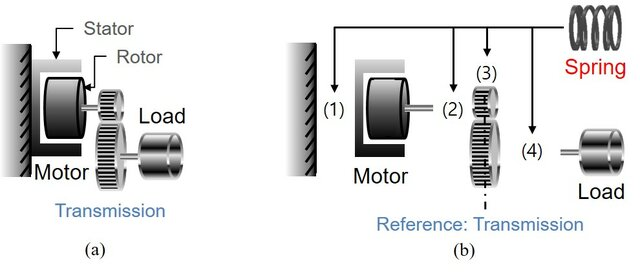
\includegraphics[width=0.95\linewidth]{SEA1}
			\caption{ Source: Lee, C., Kwak, S., Kwak, J. and Oh, S., 2017, August. Generalization of series elastic actuator configurations and dynamic behavior comparison. In Actuators (Vol. 6, No. 3, p. 26). MDPI. }
			\label{fig:sea1}
		\end{figure}
		
		
	\end{flushleft}
\end{frame}


\begin{frame}{Series-elastic actuator, 3}
	\begin{flushleft}
		
% TODO: \usepackage{graphicx} required
\begin{figure}
	\centering
	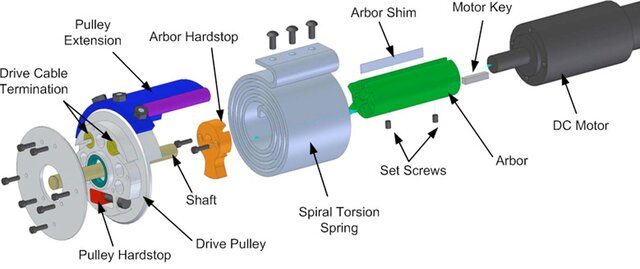
\includegraphics[width=0.95\linewidth]{SEA2}
	\caption{Source: Knox, B.T. and Schmiedeler, J.P., 2009. A unidirectional series-elastic actuator design using a spiral torsion spring.}
	\label{fig:sea2}
\end{figure}

		
	\end{flushleft}
\end{frame}


\begin{frame}{SEA electro-mechanical model, 1}
	\begin{flushleft}
		
		Full electro-mechanical model of a DC motor is:
		
		\begin{equation}
			\begin{cases}
				L \dot I + RI + C_w \omega = u \\
				J \dot \omega + F \omega = C_\tau I
			\end{cases}
		\end{equation}
	
		\bigskip
		
		For a SEA it is a little more complex:
		
		\begin{equation}
			\begin{cases}
				L \dot I + RI + C_w \dot \varphi_m = u \\
				J_m \ddot \varphi_m + F \dot \varphi_m = C_\tau I - k (\varphi_m - \varphi_o) \\
				J_o \ddot \varphi_o = k (\varphi_m - \varphi_o)
			\end{cases}
		\end{equation}
		%
		where $\varphi_m$ and $\varphi_o$ - orientations of the internal motor shaft and the output shaft, 
		$J_m$ and $J_o$ are moments of inertia of the motor and the output shaft, 
		$k$ is the stiffness of the SEA spring, 
		$L$, $R$, $C_w$, $C_\tau$, $I$, $u$ are inductance, resistance, back-EMF and torque coefficients, current and input voltage.
		
		
	\end{flushleft}
\end{frame}



\begin{frame}{SEA electro-mechanical model, 2}
	\begin{flushleft}
		
		The output torque of the SEA can be defined as:
		
		\begin{equation}
			\tau_o = k (\varphi_m - \varphi_o)
		\end{equation}
		
		This allows us to pose a control problem where control input is voltage $u$ and output is the desired torque $\tau_o$.
		
		\bigskip
		
		To achieve this type of control it might be useful (and even necessary) to measure both $\varphi_m$ and $\varphi_o$.
		
		
	\end{flushleft}
\end{frame}



\begin{frame}{Spring design}
	\begin{flushleft}
		
		% TODO: \usepackage{graphicx} required
		\begin{figure}
			\centering
			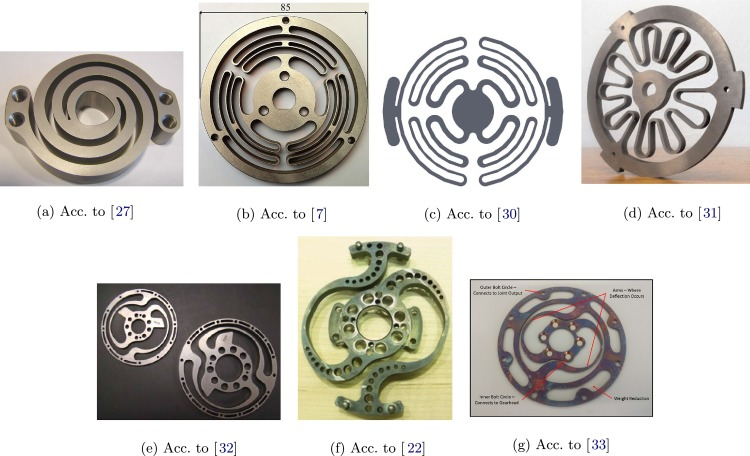
\includegraphics[width=0.9\linewidth]{SEA_spring}
			\caption{Source: Irmscher, C., Woschke, E., May, E. and Daniel, C., 2018. Design, optimisation and testing of a compact, inexpensive elastic element for series elastic actuators. Medical engineering \& physics, 52, pp.84-89.}
			\label{fig:seaspring}
		\end{figure}
		
		
		
	\end{flushleft}
\end{frame}




\begin{frame}{SEA vs spring-like control}
	\begin{flushleft}
		
		As we remember from previous lectures, we could implement such control that would make the closed-loop system behave as a spring-mass-damper. However, there are two independent reasons why this does not allow to make a DC motor with rigid gear box behave at a SEA.
		
		\bigskip
		
		First, the collision event is an instantaneous change of kinetic energy, which does not depend on control law. 
		
		\bigskip
		
		Second, the control law is discrete, meaning that at certain time-scales it will remain constant, which is not a behavior of a spring-mass-damper. Also, control law is characterized by time lag, meaning that the reaction to a collision event will start only $t_0$ seconds after the collision began. 
		
	\end{flushleft}
\end{frame}



\myqrframe

\end{document}
